\documentclass[12pt]{article}
\usepackage[utf8]{inputenc}
\usepackage[T2A]{fontenc}
\usepackage[russian]{babel}
\usepackage{amsmath}
\usepackage{graphicx}

\title{Лабораторна робота №2 \\ З курсу: Теоретико-числові алгоритми в криптології \\ Тема: Застосування алгоритму дискретного логарифмування}
\author{Анучіна Максима ФБ-11}
\date{2024}

\begin{document}

\maketitle

\section{Мета роботи}
Ознайомлення з алгоритмом дискретного логарифмування Сільвера-Поля-Хеллмана. Практична реалізація цього алгоритму. Пошук переваг, недоліків та особливостей застосування даного алгоритму дискретного логарифмування. Практична оцінка складності роботи алгоритму.

\section{Постановка задачі}
Реалізувати два алгоритми для розв'язання задачі дискретного логарифмування:
\begin{enumerate}
    \item Алгоритм повного перебору.
    \item Алгоритм Сільвера-Поля-Хеллмана.
\end{enumerate}
Для кожного алгоритму провести вимірювання часу роботи та порівняти результати.

\section{Хід роботи}
Для програмної реалізації обрано мову Python. Основною проблемою, з якою я зіткнувся, було обмеження часу виконання для великих значень параметра \( p \). Для уникнення цих обмежень було використано обробку сигналів, що дозволяє завершити програму при перевищенні часу виконання. Також при тестуванні алгоритму Сільвера-Поля-Хеллмана виникали проблеми з таблицею значень \( \beta_{q_i} \), одну з проблем вдалось вирішити завдяки заміні звичайних таблиць на хеш-таблиці, це прибрало багато помилок, але все ж таки залишась невідома мені помилка, що може бути пов'язано з обмеженнями пам'яті або ресурсів. Бо при дебазі просто не вистачало розрахункових потужностей.

\section{Результати дослідження}
Задачі мають вигляд \(x = \log_{\alpha} \beta\). У випадку перевищення часу виконання у 5 хвилин програма завершується з повідомленням "Time limit exceeded".
Задачі першого типу мають порядки, канонічний розклад яких не містить великих простих чисел. Натомість задачі другого типу мають у канонічному розкладі порядку великі прості.

Приклад запуску програми для розв’язання задачі пошуку дискретного логарифма за випадковими значеннями параметрів і до number = кількість цифр у числі:

\begin{verbatim}
docker run -it --rm discrete_log_solver --test [number] [number]
\end{verbatim}

При виконанні алгоритму Сільвера-Поля-Хеллмана виникали проблеми з таблицею значень \( \beta_{q_i} \). При деяких значеннях \( \beta_{q_i} \) програма не знаходила відповідних значень у таблиці, що викликало помилку. Це може бути пов'язано з недостатньою пам'яттю або іншими обмеженнями ресурсів. Також виникали проблеми з обчислювальною складністю при великих значеннях параметра \( p \), що призводило до перевищення часу виконання.

\begin{table}[h]
\centering
\begin{tabular}{|c|c|c|c|c|c|}
\hline
\(\alpha\) & \(\beta\) & \(p\) & Час (повний перебір) [с] & Час (С-П-Х) [с] & Результат \\ \hline
2 & 2 & 3 & 0.00002 & 0.00006 & 1 \\ \hline
5 & 4 & 11 & 0.00002 & 0.00008 & 3 \\ \hline
3 & 7 & 13 & 0.00002 & - & None \\ \hline
74 & 39 & 101 & 0.00007 & 0.00006 & 55 \\ \hline
44 & 32 & 103 & 0.00007 & 0.00007 & 98 \\ \hline
327 & 885 & 1009 & 0.00088 & 0.00011 & None \\ \hline
521 & 261 & 1013 & 0.00087 & 0.00006 & None \\ \hline
8636 & 5322 & 10007 & 0.00535 & 0.00449 & 5968 \\ \hline
4669 & 1470 & 10009 & 0.00168 & 0.00020 & 1946 \\ \hline
21531 & 95502 & 100003 & 0.00826 & 0.00287 & 7874 \\ \hline
9280 & 15399 & 100019 & 0.02747 & 0.00153 & 26159 \\ \hline
688979 & 830890 & 1000003 & 0.23991 & 0.21984 & 182560 \\ \hline
200489 & 366465 & 1000033 & 1.43864 & 0.00014 & None \\ \hline
4229237 & 6325732 & 10000019 & 2.62054 & 0.00212 & 1788724 \\ \hline
3512346 & 3514593 & 10000079 & 0.90222 & 0.02313 & 647801 \\ \hline
66112151 & 65563534 & 100000007 & 0.03023 & 0.00287 & 24175 \\ \hline
51033572 & 45973358 & 100000037 & 1.73027 & 0.00014 & 1088180 \\ \hline
\end{tabular}
\caption{Результати вимірювання часу роботи алгоритмів}
\end{table}

\section{Оцінка максимального порядку}
Максимальний порядок параметра \( p \), при якому процес побудови задачі і її розв'язання відбувався за відведений час, склав \( p = 100000037 \) для алгоритму повного перебору та значно менші значення для алгоритму Сільвера-Поля-Хеллмана.

\section{Висновки}
Метою лабораторної роботи було ознайомлення з алгоритмом дискретного логарифмування Сільвера-Поля-Хеллмана. Було реалізовано два алгоритми для розв'язання задачі дискретного логарифмування та проведено порівняльний аналіз їх продуктивності. Алгоритм повного перебору показав стабільну роботу для всіх значень параметра \( p \), тоді як алгоритм Сільвера-Поля-Хеллмана зіткнувся з проблемами при великих значеннях \( p \), що може бути пов'язано з обмеженнями пам'яті або ресурсів.

Вихідний код реалізованої програми розміщено на платформі GitHub за посиланням (https://github.com/deathmaks/NTA2).
Docker-контейнер з реалізованою програмою доступний за посиланням

(https://hub.docker.com/r/anmatos/discrete-log-solver).(P.S. потрібно замінити - на нижній дефіс)

\begin{figure}[h]
\centering
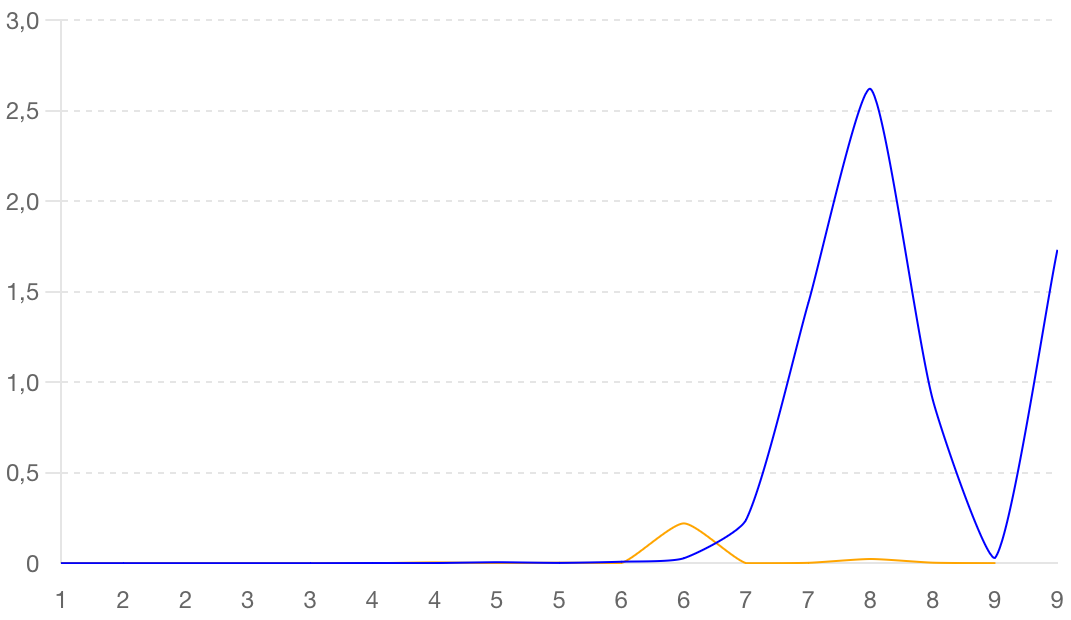
\includegraphics[width=0.8\textwidth]{time.png}
\caption{Залежність часу роботи алгоритмів від параметра \( p \)}
\end{figure}

\section{Оцінка максимального порядку}
Максимальний порядок параметра \( p \), при якому процес побудови задачі і її розв'язання відбувався за відведений час, склав \( p = 1000000007 \).

\end{document}
